% !TeX root = ../main.tex

\chapter{需求分析}

\section{整体需求}

随着机器学习、深度学习与人工智能的发展,智能文档及其语料处理的需求逐渐增加。

通用文档处理不仅需要识别文档中图表、图片、表格等信息,还包括对其他形式文档的还原,
包括对语料中蕴含的实体进行正确的提取和解析,并将其数据形式结构化。
本项目着重于文档语料中的实体识别与解析,尤其是其中的时间表达式信息抽取。

中文时间表达式信息抽取的研究已经经历了较长一段时间,
目前也取得了一定的进展,但就目前市场或开源项目中的中文时间信息抽取系统而言,并不能令人满意。
究其原因,不仅因为中文本身的表现形式复杂,并且对于时间的概念也存在着缺省描述,
同时也没有统一的标注方式和大量的训练语料,导致大部分的解决方案只能做到识别,而不能兼顾对时间表达式的解析。
所以本中文时间表达式信息抽取系统需要在正确识别中文时间表达式的基础之上,
进一步满足中文时间表达式解析功能的需求,
同时需要搭配相应的接口(API,Application Programming Interface)和用户界面(UI,User Interface),实现工程化场景落地。

中文时间表达式识别,需要准确提取出语料中的实体部分,
标出识别到的中文时间表达式的左右边界,特定情况下,还需要分别标识一个时间表达式内部的基本元素的边界,这部分遵循实体抽取的一般步骤。

时间表达式识别的市场需求很大,因此不仅有各大互联网企业的平台在研究中文时间表达式,如阿里云小蜜平台、讯飞开放平台、百度Unit平台等,还有很多中小企业在致力于中文时间表达式识别的研究,如美能华智能科技的智能文档处理平台。

中文时间表达式的解析,需要将识别出来的实体部分通过一定的方法或者算法进行转化,最终归一化成某种时间格式,在本中文时间表达式信息抽取中采用的是协调世界时(UTC,Coordinated Universal Time)。时间表达式解析也被广泛使用在其他NLP(Nature Lauguage Processing)任务中,现代搜索引擎譬如必应搜索引擎基于时间表达式解析直接生成问题对应答案,虚拟语音助手譬如微软Cortana和亚马逊Alexa等结合表格和自然语言理解技术回答用户语音请求。此外,时间表达式解析可使用在检索、对话、问题生成等一系列NLP任务中。

\begin{figure}[h]
    \centering
    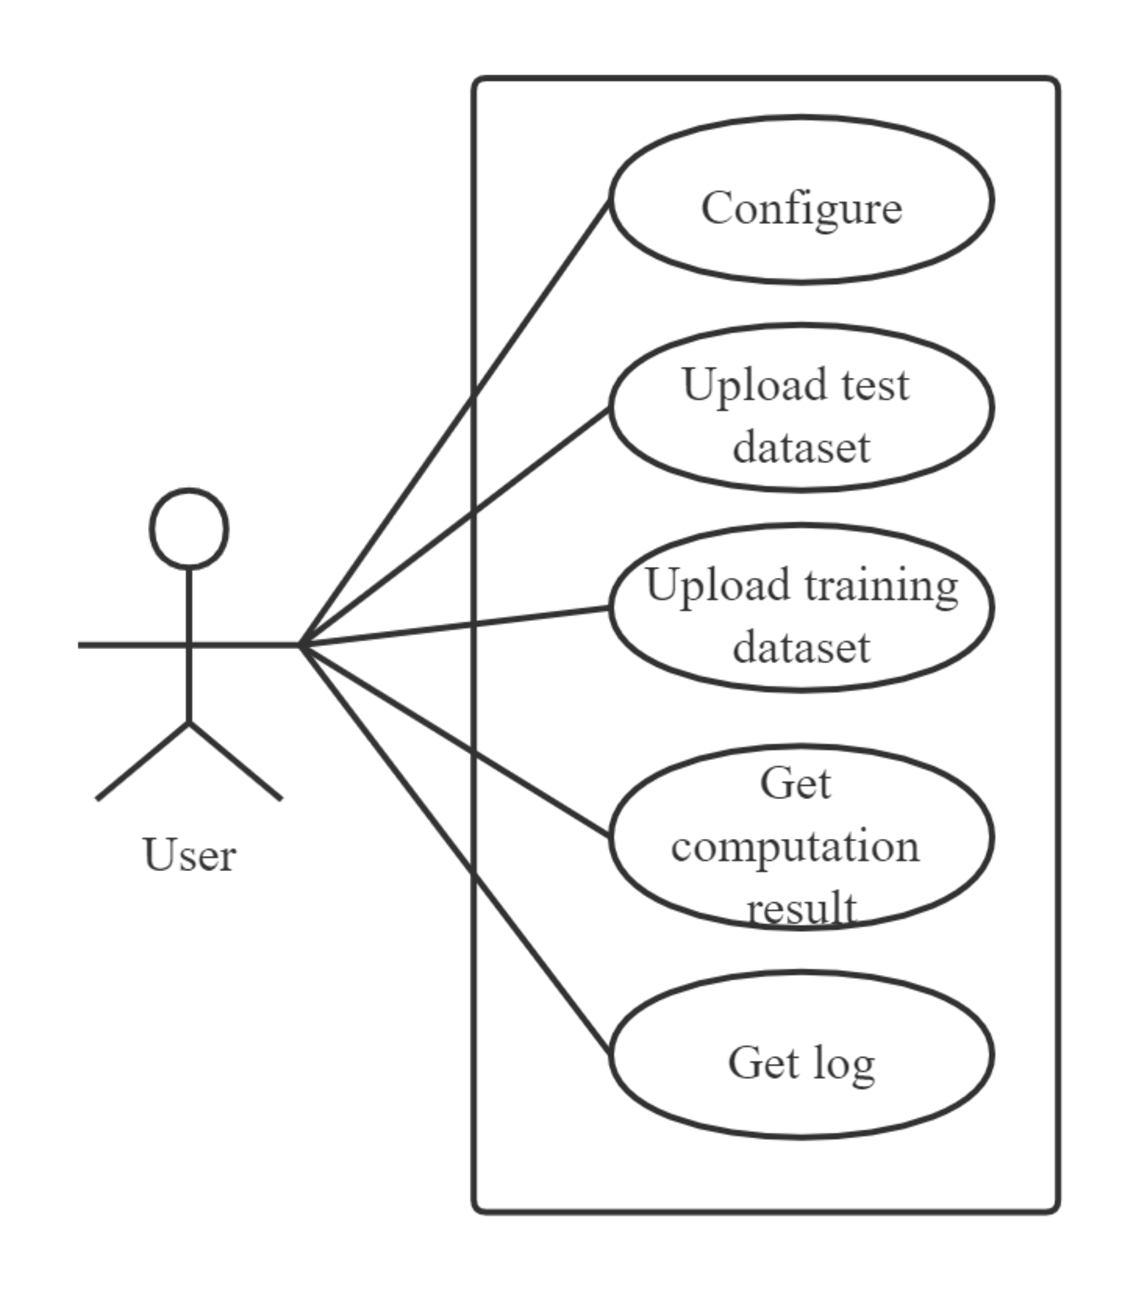
\includegraphics[width=0.7\textwidth]{usercase.pdf}
    \caption{用户用例图}
    \label{fig:usecase}
\end{figure}

\section{功能性需求}

功能需求部分主要阐述中文时间表达式信息抽取系统设计所要实现的目标,分析系统各个模块的功能和具体实现方式。
本文以用例图直观展示系统需求,以下从用户和开发者角度介绍系统。

在中文时间表达式信息抽取系统中,会提供一个用户界面使得用户根据自身需要,选择需要识别的时间数据类型或时间表达式解析后推荐的结果数量,根据选择的配置,下载或导入训练数据与测试数据。
当用户界面将上述的时间数据类型、结果推荐数、训练数据与测试数据导入时间抽取模块之后,时间抽取模块会根据用户导入的或系统默认的训练数据训练时间信息识别模块。
当时间信息模块训练完成后,便对用户导入的测试数据进行测试,并通过时间信息归一化模块对识别的结果进行计算。
在时间抽取模块的计算过程完成后,会将整体计算结果在用户界面展示,同时用户也可下载日志数据观察详细的计算过程。
同时数据存储层会将用户的训练数据,测试数据,计算结果等保存在数据库中。用户用例图如图~\ref{fig:usecase}所示。

图~\ref{fig:develope_usecase}为系统的开发者用例图,针对开发者而言需要设计中文时间表达式识别和解析两个模块,同时需要配置用户服务接口。

针对识别和解析部分,我们还需要搭配朴素贝叶斯选择器模块以消除中间过程可能产生的歧义问题。
对于用户界面,首先需要设计上传功能以获取用户传入的语料或者文档,必要情况下还需要使用辅助的文字转化功能,如OCR功能以识别PDF文档中的文字。
表达式识别与解析模块将处理后的语料作为识别和解析模块的输入,最终产生用户所需要的数据格式。
用户上传的数据以及已有的训练语料都应该存放于数据库之中,便于开发人员纠错以及再训练。

\begin{figure}[h]
    \centering
    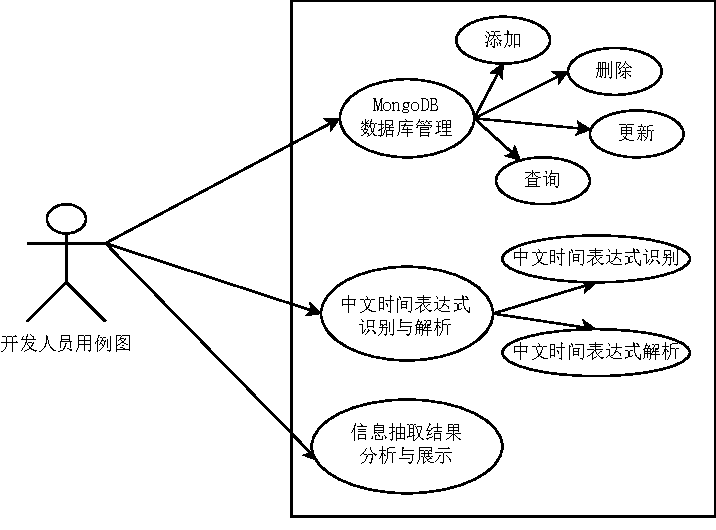
\includegraphics[width=0.8\textwidth]{develop_usercase.pdf}
    \caption{开发人员用例图}
    \label{fig:develope_usecase}
\end{figure}

\subsection{中文时间表达式识别模块}

中文时间表达式识别模块旨在从文档或语料中获取相关的实体,并标名实体在语料中的范围,因此识别模块的功能需求如下所示:
\begin{enumerate}
    \item[(1)] 模块输入不仅能支持普通的文本类型输入,还需要支持PDF文档以及图片或图片格式的PDF文档,并且输出为文本形式;
    \item[(2)] 模块必须要准确无歧义的识别到具体的实体,并以区间的形式标明时间表达式在语料中的具体位置。
\end{enumerate}

\subsection{中文时间表达式解析模块}

中文时间表达式解析模块是根据从识别模块中获取到的实体及实体范围等信息,解析成UTC时间格式,以便其他任务需要。
因此中文时间表达式解析模块的功能性需求如下所示:
\begin{enumerate}
    \item[(1)] 将识别到的实体转换为UTC时间格式,并返回给用户;
    \item[(2)] 为了便于用户理解,需要将实体解析过程中形成的解析树以可视化的形式呈现给用户;
    \item[(3)] 除了返回最终的UTC时间格式的结果,还需要提供时间解析的备选方案给用户,方便用户及时反馈并纠错;
\end{enumerate}

\subsection{相关接口}

对于用户来说,不会关心模型的中间处理步骤,只会关系模型的输出结果,因此为了使用户方便得到结果,需要相关接口进行数据可视化,那么需要满足以下要求:
\begin{enumerate}
    \item[(1)] 输出数据的通用化,对于用户输入,若其形式为图片或PDF文档,应该返回文本形式的语料,并附上相应的信息,包括识别到的时间表达式,时间表达式在语料中的具体位置,以及时间表达式归一化为UTC时间格式后的字符串,并将返回数据组织为文档形式,方便用户下载;
    \item[(2)] 若用户是通过单句语料输入的,则输出数据的中间结果需要可视化为树形结构,并在用户界面展示;
    \item[(3)]  用户调用,对于系统的使用,需要规定相关的接口,对服务器进行配置,通过网络请求返回结果。
\end{enumerate}

\section{非功能性需求}

中文时间表达式信息抽取模块在满足功能需求的基础之外,还需要根据具体的使用情况满足非功能性方面的需求。
中文时间表达式信息抽取系统应用的非功能需求,体现在系统的准确性、系统的实施性、系统的可扩展性和系统的可维护性。
任何一个软件想要持续的生存下去,这些性能指标都是不可获取的。只有同时满足功能性需求和非功能性需求,该中文时间表达式信息抽取系统才是完整的。

\subsection{准确性}

本中文时间表达式信息抽取系统的准确性是决定项目价值的最重要的因素。
识别模块和解析模块的任意部分出错都会造成最终结果的不准确,导致大量的遗漏或者错误解析。
识别结果的遗漏会显著降低识别模块的可信力,链式的减少解析模块对最终结果的掌握权,导致用户无法信任中文时间表达式信息抽取结果的全面性;
错误解析会带来更严重的后果,如果将某些不属于时间表达式的部分语句解析成正确的结果,或者无法正确分析时间表达式并将其输出结果,那么不仅会让用户对结果感到不满,也会对开发人员的处理过程造成极大的干扰。
参考多篇文献及相关的工程项目或开源项目,本中文时间表达式信息抽取系统要求识别过程应该至少达到90\%,而解析准确度在识别成功的基础上,应该至少达到85\%。

\subsection{实时性}

对于本中文时间表达式信息抽取系统的实时识别与解析功能来讲,优质的交互性体验也是重要的一环。
这就要求本中文时间表达式信息抽取系统从接收用户输入,再经过识别与解析,最后生成可视化视图返回用户的时间应该尽可能处于较短的水平,使整个交互过程满足用户的接受范围之内。
因此本项目在本地上进行单句语料的信息抽取时间应该控制在毫秒级别。
在远程调用的场景下,由于需要依赖额外的服务器资源的支持,则尽可能将单句语料的信息抽取时间控制在毫秒到秒级别。
随着语料内容量级性的增长,最终的响应时间控制为成线性增长。

\subsection{可扩展性}

中文时间表达式的识别模块定义了许多基本的识别元素,这些基本的元素相互独立,耦合性较低。
在添加新的识别规则时,开发人员可以根据这些基本的识别元素相互组合,也可以定义新的基本元素,当元素或者组合元素与原有的识别规则冲突时,
识别模块会自动报道相关的规则冲突。

\subsection{可维护性}

软件开发过程并不是一蹴而就、一劳永逸的。项目初步完成之后,还需要经历多个版本的迭代、验证和再迭代。
后续开发过程仍然需要不断的维护,才能保证软件本身的稳定性和可用性。
在本中文时间表达式信息抽取系统的开发中,规则和基本元素的开发人员需尽量保持独立。
本项目不仅需要保证组件之间耦合程度低,接口清晰简单,以利于后续的维护工作。其次,保证系统模块清晰、代码整洁度高、可读性强、没有冗余代码。

\subsection{可兼容性}

兼容性也是评价一个软件非功能性需求的一个重要指标,软件具有良好的兼容性才能部署到各种平台,从而拥有广泛的使用群体; 同时良好的兼容性也避免了项目部署到服务端造成的差异化问题。
% 如果软件只局限于某一个平台下使用,必然会限制本中文时间表达式信息抽取系统的用户范围。
% (tips:删掉后面的,放在测试里)本系统的实现在语言上依赖于Python,而工具包仅依赖于scikit-learn,将所有的需求环境打包后能够同时支持在Linux操作系统和Windows操作系统上部署并稳定运行。用户可以通过RESTFul的风格传入语料,在自己熟悉的环境下使用本中文时间表达式信息抽取系统。本系统保证良好的兼容性。

\section{本章小结}

本章节从实际需求出发,根据该中文时间表达式信息抽取系统的应用场景,详细分析了该信息抽取系统的功能性需求以以非功能性需求。
在功能需求方面,本章节详细描述了该系统的主要功能,即本项目需要实现中文时间表达式的识别与解析两种功能。
同时为了提高用户体验,另外设计了可视化的树形解析结果,帮助用户和开发人员校验解析结果的可行性。
在非功能性需求方面,本系统着重分析了准确性与实时性两点,同时阐述了中文时间表达式信息抽取系统在可兼容性、可扩展性和可维护性等方面的具体需求。
本章对中文时间表达式信息抽取系统的功能性以及非功能性需求,为下文中的概要设计建立了良好的基础。
